\chapter{Описание принципа работы подсистемы измерения энергопотребления}
\section{Обоснование выбора компонентов измерительной части}
\subsection{Операционный усилитель}
\hspace{1cm} 

Вопрос какой операционный усилитель (далее ОУ) использовать в качестве дифференциального усилителя -- самый 
критичный для подсистемы измерения энергопотребления. Прежде всего стоит определиться с требованиями к 
самым важным параметрам ОУ. 
Одной из важных характеристик операционного усилителя (ОУ) является напряжение смещения $V_{os}$ — или, 
говоря проще, напряжение ошибки на его входах. Любой неидеальный ОУ при отсутствии входного сигнала выдаёт 
выходной так, как будто бы на самом деле вход-ной сигнал равен Vos.

Напряжение смещения обычно составляет от единиц микровольт до единиц милливольт — и, соответственно, 
доставляет серьёзные неудобства при работе с низковольтными источни-ками: термопарами, шунтами и так далее.
Особенно — если оно отрицательное, а схема однополярная: тогда на выходе ОУ будет просто 0, пока 
напряжение входного сигнала не превысит Vos, и никакой калибровкой это устранить невозможно \cite{Chopper:OU} 
\cite{MT-037:Tutorial}. 

При измерении микро- и милиамперных диапазонов высокое напряжение смещение мо-жет стать проблемой.
Для этого следует изучить реальную зависимость напряжения смещения от Vcm и сравнить ее с той, 
которую приводят в datasheet, как, например, на рисунке \ref{ris:411} \cite{OPAx376:datasheet}.
\begin{figure}[H]
\centering
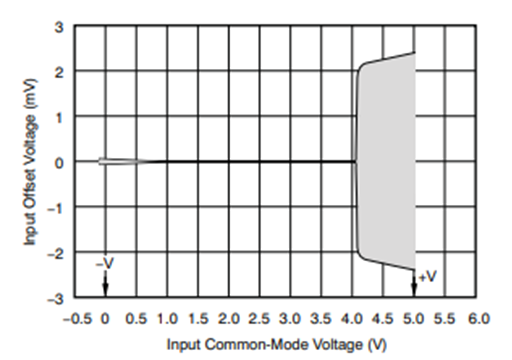
\includegraphics[scale = 1]{ris411.png}
\caption{Зависимость напряжения смещения от $V_{cm}$}
\label{ris:411}
\end{figure}

Так же стоит посмотреть на напряжение смещения в зависимости от ОУ в партии, 
на рисунке \ref{ris:412} представлен график для OPA2376 \cite{OPAx376:datasheet}

\begin{figure}[H]
\centering
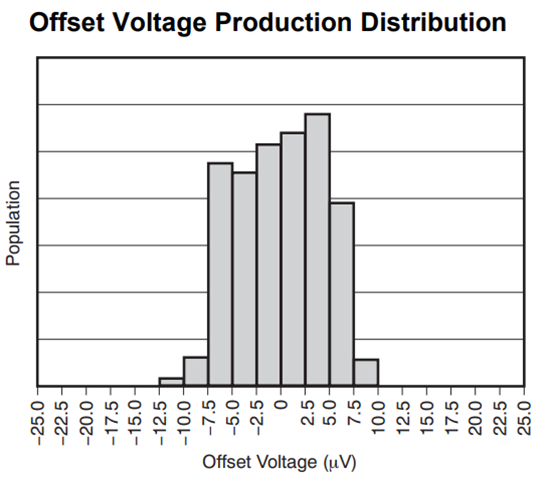
\includegraphics[scale = 1]{ris412.png}
\caption{Показатель напряжения смещения в рамках одной партии}
\label{ris:412}
\end{figure}

Также стоит упомянуть про то, что при использовании автоматического переключения шунтов 
чоппер-стабилизированные ОУ малопригодны из-за долгого времени восстановления, так как из-за частоты работы
АЦП порядка сотен кГц, время переключения свыше 1 мкс нам не подходит \cite{Chopper:OU}.

Исходя из вышесказанного, можно изучить следующие ОУ:

\begin{itemize}
    \item OPA2376 от Texas Instruments -- прецизионный rail-to-rail, выполненный по технологии etrim
    \item OPA2376 от Fulihao -- прецизионный rail-to-rail, выполненный по технологии etrim
    \item AD8606 от Analoc Device -- прецизионный rail-to-rail, выполненный по технологии etrim
    \item TP2312 -- прецизионный малошумящий rail-to-rail
    \item RS8552 -- чоппер-стабилизированный
    \item RS8562 -- чоппер-стабилизированный
\end{itemize}

На выбор ОУ влияла так же возможность быстро и без проблем приобрести на территории РФ. 

На рисунке \ref{ris:413} представлена схема измерения напряжения смещения.

\begin{figure}[H]
    \centering
    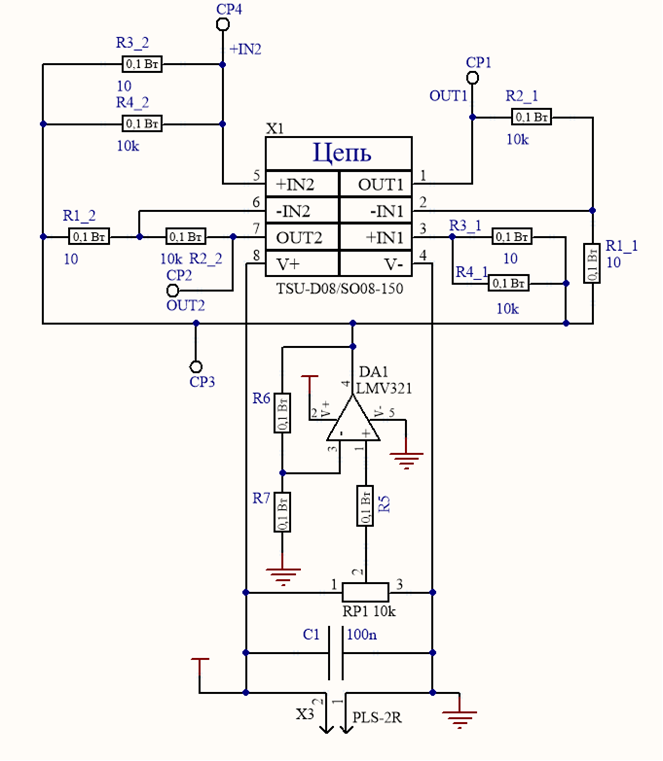
\includegraphics[scale = 0.9]{ris413.png}
    \caption{Схема измерительной установки}
    \label{ris:413}
    \end{figure}

Здесь Х1 -- контактирующее устройство, предназначенное для быстрой смены операци-онного усилителя в 
корпусе SOIC-8 -- самого распространённого типа корпуса для ОУ. Испытуемый ОУ включён по схеме неинвертирующего 
усилителя с коэффициентом усиления 1000, который обеспечивается резисторами R2\_1 и R1\_1 для первого ОУ и
резисторами R2\_2 и R1\_2 для второго ОУ в корпусе. DA1 с обвязкой к нему выполняет роль буферного ОУ для 
обеспечения лучшего импеданса и большей нагрузочной способности при низком токе через делитель R3 и R4.

Данная схема позволит преобразовать микровольтное напряжение смещение в миливольты, что достаточно для 
измерения обычным вольтметром. Подстроечным резистором RP1 регулируется input common-mode voltage, как 
на рисунке \ref{ris:411}. Напряжение питание схемы 5 В.

% Table generated by Excel2LaTeX from sheet 'Vcm' and from my teardrops
\begin{table}[H]
    \begin{adjustwidth}{-1em}{}
    \centering
    \caption{Результаты измерений напряжения смещения у разных ОУ}
      \begin{tabular}{|c|c|c|c|c|c|c|c|c|c|c|c|}
      \hline
      \multicolumn{1}{|c|}{\multirow{3}[6]{2cm}{\textbf{Тип ОУ}}} & \multicolumn{1}{c|}{\multirow{3}[6]{1.4cm}{\textbf{Номер экземпляра}}} & \multicolumn{1}{c|}{\multirow{3}[6]{1.8cm}{\textbf{Номер ОУ в корпусе}}} & \multicolumn{9}{|c|}{\textbf{Напряжение смещения, мВ}} \bigstrut\\
  \cline{4-12}          &       &       & \multicolumn{9}{|c|}{\textbf{При Vcm, В}} \bigstrut\\
  \cline{4-12}          &       &       & \textbf{0,5} & \textbf{1} & \textbf{1,5} & \textbf{2} & \textbf{2,5} & \textbf{3} & \textbf{3,5} & \textbf{4} & \textbf{4,5} \bigstrut\\
      \hline
      \multicolumn{1}{|c|}{\multirow{10}[20]{*}{OPA2376 }} & \multirow{2}[4]{*}{1} & 1     & 13,4  & 7,9   & 2,4   & -2,4  & -8,1  & -11,8 & -15,3 & -12,8 & 483 \bigstrut\\
  \cline{3-12}          &       & 2     & 4,2   & 6     & 4,3   & 2,3   & -1    & -3,5  & -6    & -9,7  & -1813 \bigstrut\\
  \cline{2-12}          & \multirow{2}[4]{*}{2} & 1     & 28,5  & 18,7  & 9,3   & 0,3   & -8    & -15,2 & -22,7 & -58,5 & -388 \bigstrut\\
  \cline{3-12}          &       & 2     & -5,5  & -7,5  & -8,5  & -6,8  & -6,1  & -3,9  & -1,9  & -8,9  & -680 \bigstrut\\
  \cline{2-12}          & \multirow{2}[4]{*}{3} & 1     & 26,7  & 20,3  & 14,2  & 9,1   & 3,6   & -0,2  & -4,4  & -16,6 & -2230 \bigstrut\\
  \cline{3-12}          &       & 2     & -55,7 & -33,4 & -21,7 & -12,3 & -7,3  & -1,5  & 2,9   & -10,9 & -4500 \bigstrut\\
  \cline{2-12}   TI     & \multirow{2}[4]{*}{4} & 1     & -18,2 & -10,8 & -6,3  & -2,5  & 0,1   & 2,5   & 4,6   & 14,5  & -1532 \bigstrut\\
  \cline{3-12}          &       & 2     & 7,2   & 5,5   & -0,1  & -4,8  & -9,2  & -13,4 & -17,2 & -23,3 & -1517 \bigstrut\\
  \cline{2-12}          & \multirow{2}[4]{*}{5} & 1     & -18,8 & -10,4 & -4,5  & 0,2   & 3,2   & 6,3   & 8,6   & 22    & 395 \bigstrut\\
  \cline{3-12}          &       & 2     & -70,4 & -43,6 & -24,7 & -11,2 & -1,6  & 7,5   & 14,4  & 30    & 624 \bigstrut\\
      \hline
      \multicolumn{1}{|c|}{\multirow{6}[12]{*}{OPA2376}} & \multirow{2}[4]{*}{1} & 1     & -6,3  & -6,5  & -8,4  & -8,2  & -7,35 & -7,9  & -10   & -5,9  & -4,6 \bigstrut\\
  \cline{3-12}          &       & 2     & -2,8  & -2,9  & -4,5  & -4,3  & -3,1  & -3,3  & -4,7  & -2,7  & -1,7 \bigstrut\\
  \cline{2-12}          & \multirow{2}[4]{*}{2} & 1     & -6,8  & -6,8  & -9    & -9    & -8,01 & -8,9  & -10,4 & -11,8 & -10,1 \bigstrut\\
  \cline{3-12}          &       & 2     & 1,3   & 1     & -0,6  & -0,5  & 0,2   & 1,2   & -0,1  & 2     & 3,4 \bigstrut\\
  \cline{2-12} Fulihao   & \multirow{2}[4]{*}{3} & 1     & -4,6  & -4,4  & -6,4  & -6,8  & -6,4  & -6,5  & -8,5  & -7,7  & -6,2 \bigstrut\\
  \cline{3-12}          &       & 2     & -1,4  & -1,2  & -2,3  & -2,1  & -0,8  & -0,6  & -2,3  & -1,5  & 0,2 \bigstrut\\
      \hline
      \multicolumn{1}{|c|}{\multirow{10}[20]{*}{AD8606}} & \multirow{2}[4]{*}{1} & 1     & 40,1  & 36,3  & 33,7  & 33,5  & 31,3  & 30,6  & 3,5   & 6,2   & 19,8 \bigstrut\\
  \cline{3-12}          &       & 2     & 11,4  & 32,8  & 49,3  & 59,67 & 72    & 80,5  & 19,2  & -10,4 & -13,6 \bigstrut\\
  \cline{2-12}          & \multirow{2}[4]{*}{2} & 1     & 21,4  & 27,2  & 31,3  & 34,5  & 36,1  & 38,3  & 87,5  & 73,8  & 93,6 \bigstrut\\
  \cline{3-12}          &       & 2     & 12,8  & 4,6   & 0,6   & -0,3  & -2,2  & -2,1  & -94,4 & -39,9 & -46,5 \bigstrut\\
  \cline{2-12}          & \multirow{2}[4]{*}{3} & 1     & 17,8  & 34,3  & 47,5  & 59,2  & 71,8  & 84,9  & 29,7  & 29,5  & 23,6 \bigstrut\\
  \cline{3-12}          &       & 2     & -16,3 & -3,3  & 6,6   & 13,9  & 1,3   & 27,9  & 48,8  & 9,3   & 15,6 \bigstrut\\
  \cline{2-12}          & \multirow{2}[4]{*}{4} & 1     & 74,7  & 63,5  & 51,1  & 40,5  & 31,9  & 24,1  & 40,9  & 61,6  & 73,7 \bigstrut\\
  \cline{3-12}          &       & 2     & 15,3  & -6,9  & -25,1 & -38,5 & -51,4 & -64,2 & -53,8 & -17,5 & -29,4 \bigstrut\\
  \cline{2-12}          & \multirow{2}[4]{*}{5} & 1     & 59,5  & 51,8  & 41,9  & 35,3  & 24,8  & 18,3  & 10,4  & 0,9   & 11,8 \bigstrut\\
  \cline{3-12}          &       & 2     & 14,9  & 22,5  & 32,1  & 37,4  & 44,2  & 48,6  & 35,2  & 35,7  & 40,4 \bigstrut\\
      \hline
      \multicolumn{1}{|c|}{\multirow{10}[20]{*}{TP2312}} & \multirow{2}[4]{*}{1} & 1     & 17,4  & 18,2  & 18,8  & 20,6  & 23,3  & 26,5  & 28,9  & 165,9 & -1072 \bigstrut\\
  \cline{3-12}          &       & 2     & 30,4  & 38,6  & 43,6  & 47,9  & 49,7  & 50,6  & 51,2  & -41,7 & -1550 \bigstrut\\
  \cline{2-12}          & \multirow{2}[4]{*}{2} & 1     & -12,4 & -10,2 & -7    & -2,6  & 3,2   & 7     & 12,9  & -391  & -3330 \bigstrut\\
  \cline{3-12}          &       & 2     & 8,3   & 14,9  & 19,3  & 22,4  & 26,9  & 30,8  & 34,2  & 24,3  & -1183 \bigstrut\\
  \cline{2-12}          & \multirow{2}[4]{*}{3} & 1     & 12,8  & 6,6   & 2,3   & -4,2  & -10,9 & -16,9 & 46,3  & 34,9  & -403 \bigstrut\\
  \cline{3-12}          &       & 2     & 16,2  & 15,4  & 17,1  & 19,4  & 23    & 27,5  & 51,2  & 330   & -1491 \bigstrut\\
  \cline{2-12}          & \multirow{2}[4]{*}{4} & 1     & -24,1 & -16,9 & -11   & -4,3  & 0,5   & 4,1   & 8,4   & 269   & -2530 \bigstrut\\
  \cline{3-12}          &       & 2     & 3,7   & 3,9   & 4,5   & 6,8   & 9,1   & 12,9  & 16,7  & 468   & -1950 \bigstrut\\
  \cline{2-12}          & \multirow{2}[4]{*}{5} & 1     & 3,6   & -13,8 & -23,8 & -31,8 & -38,5 & -43,8 & -47,3 & -123,2 & -2660 \bigstrut\\
  \cline{3-12}          &       & 2     & 28,2  & 23    & 18,5  & 14    & 8,8   & 5,3   & 1,3   & 934   & -171 \bigstrut\\
      \hline
      \end{tabular}%
    \label{tab:Vcm1}%
    \end{adjustwidth}
  \end{table}



  \begin{table}[H]
    %\begin{adjustwidth}{-2em}{}
    \centering
    \caption{Результаты измерений напряжения смещения у разных ОУ}
      \begin{tabular}{|c|c|c|c|c|c|c|c|c|c|c|c|}
      \hline
      \multicolumn{1}{|c|}{\multirow{3}[6]{2cm}{\textbf{Тип ОУ}}} & \multicolumn{1}{c|}{\multirow{3}[6]{1.4cm}{\textbf{Номер экземпляра}}} & \multicolumn{1}{c|}{\multirow{3}[6]{1.8cm}{\textbf{Номер ОУ в корпусе}}} & \multicolumn{9}{|c|}{\textbf{Напряжение смещения, мВ}} \bigstrut\\
  \cline{4-12}          &       &       & \multicolumn{9}{|c|}{\textbf{При Vcm, В}} \bigstrut\\
  \cline{4-12}          &       &       & \textbf{0,5} & \textbf{1} & \textbf{1,5} & \textbf{2} & \textbf{2,5} & \textbf{3} & \textbf{3,5} & \textbf{4} & \textbf{4,5} \bigstrut\\
      \hline
      \multicolumn{1}{|c|}{\multirow{10}[20]{*}{RS8552}} & \multirow{2}[4]{*}{1} & 1     & -0,1  & -0,4  & -0,5  & 0,3   & -0,6  & -0,4  & 0,9   & -0,8  & -0,5 \bigstrut\\
  \cline{3-12}          &       & 2     & -1,3  & -0,5  & -0,4  & -0,1  & -0,5  & 0,6   & -0,2  & -0,2  & -0,9 \bigstrut\\
  \cline{2-12}          & \multirow{2}[4]{*}{2} & 1     & -0,3  & -0,4  & -0,1  & -0,4  & -0,2  & -0,3  & -0,2  & -0,6  & -5 \bigstrut\\
  \cline{3-12}          &       & 2     & -0,4  & -0,2  & 0     & -0,1  & -0,8  & -0,5  & -0,3  & -0,5  & -0,5 \bigstrut\\
  \cline{2-12}          & \multirow{2}[4]{*}{3} & 1     & -0,5  & 0,5   & 0,2   & -0,6  & -0,2  & -0,9  & -0,7  & -0,3  & -0,4 \bigstrut\\
  \cline{3-12}          &       & 2     & -0,3  & -0,6  & -0,3  & -0,2  & -0,3  & -0,2  & -0,8  & -0,4  & -0,5 \bigstrut\\
  \cline{2-12}          & \multirow{2}[4]{*}{4} & 1     & 0,8   & 1,1   & 1,4   & 1     & 0,8   & -0,7  & -0,1  & -0,6  & -0,3 \bigstrut\\
  \cline{3-12}          &       & 2     & -0,6  & -0,4  & -0,6  & -0,2  & -0,4  & -0,3  & -0,1  & -0,7  & -0,9 \bigstrut\\
  \cline{2-12}          & \multirow{2}[4]{*}{5} & 1     & -0,4  & 0,1   & -0,4  & -0,1  & -0,2  & -0,2  & -0,3  & -0,5  & -0,4 \bigstrut\\
  \cline{3-12}          &       & 2     & -0,3  & -0,3  & -0,2  & -0,5  & -0,2  & -0,1  & -0,6  & -0,5  & -0,6 \bigstrut\\
      \hline
      \multicolumn{1}{|c|}{\multirow{10}[20]{*}{RS8562}} & \multirow{2}[4]{*}{1} & 1     & -1,3  & -0,6  & -0,4  & -0,3  & -0,1  & -0,9  & -0,4  & -0,6  & -0,1 \bigstrut\\
  \cline{3-12}          &       & 2     & -1,3  & -0,4  & -0,9  & -0,5  & -0,8  & -0,3  & -0,4  & -0,8  & -0,7 \bigstrut\\
  \cline{2-12}          & \multirow{2}[4]{*}{2} & 1     & 0,1   & 0,5   & 0,1   & -0,6  & 0,5   & -0,2  & -0,2  & -0,2  & 0,3 \bigstrut\\
  \cline{3-12}          &       & 2     & -1,2  & -0,9  & -1    & -0,5  & -0,2  & -0,9  & -0,2  & -0,5  & -0,8 \bigstrut\\
  \cline{2-12}          & \multirow{2}[4]{*}{3} & 1     & 0     & 0,3   & 0,2   & -0,2  & 0,6   & -0,8  & -0,7  & -0,6  & 0,4 \bigstrut\\
  \cline{3-12}          &       & 2     & -0,8  & -0,1  & -1,2  & -0,1  & -0,1  & -0,4  & -0,6  & -0,6  & -0,9 \bigstrut\\
  \cline{2-12}          & \multirow{2}[4]{*}{4} & 1     & 0,2   & 0,6   & -0,3  & -0,7  & -0,2  & -0,9  & -0,7  & -0,2  & -0,1 \bigstrut\\
  \cline{3-12}          &       & 2     & -1,8  & -1,5  & -2,1  & -0,6  & -0,6  & -0,1  & -0,7  & -0,4  & -0,8 \bigstrut\\
  \cline{2-12}          & \multirow{2}[4]{*}{5} & 1     & -0,1  & 0,2   & 0,4   & -0,9  & 0,3   & -0,6  & -0,8  & 0,1   & -0,6 \bigstrut\\
  \cline{3-12}          &       & 2     & -1,6  & -1    & -0,6  & -0,4  & -0,5  & -0,9  & -0,1  & -0,9  & -0,7 \bigstrut\\
      \hline
      \end{tabular}%
    \label{tab:Vcm2}%
    %\end{adjustwidth}
  \end{table}
%\end{landscape}
В данной таблице результаты измерения после усиления напряжения смещения в 1000 раз. Из результатов измерений
можно сказать, что заявленное производителями напряжение смещения соответствует измеренным


\section{Расчет элементов схемы}
\hspace{1cm} 

\section{Результаты тестирования}
\hspace{1cm} 